\documentclass{article}\usepackage[]{graphicx}\usepackage[]{color}
%% maxwidth is the original width if it is less than linewidth
%% otherwise use linewidth (to make sure the graphics do not exceed the margin)
\makeatletter
\def\maxwidth{ %
  \ifdim\Gin@nat@width>\linewidth
    \linewidth
  \else
    \Gin@nat@width
  \fi
}
\makeatother

\definecolor{fgcolor}{rgb}{0.345, 0.345, 0.345}
\newcommand{\hlnum}[1]{\textcolor[rgb]{0.686,0.059,0.569}{#1}}%
\newcommand{\hlstr}[1]{\textcolor[rgb]{0.192,0.494,0.8}{#1}}%
\newcommand{\hlcom}[1]{\textcolor[rgb]{0.678,0.584,0.686}{\textit{#1}}}%
\newcommand{\hlopt}[1]{\textcolor[rgb]{0,0,0}{#1}}%
\newcommand{\hlstd}[1]{\textcolor[rgb]{0.345,0.345,0.345}{#1}}%
\newcommand{\hlkwa}[1]{\textcolor[rgb]{0.161,0.373,0.58}{\textbf{#1}}}%
\newcommand{\hlkwb}[1]{\textcolor[rgb]{0.69,0.353,0.396}{#1}}%
\newcommand{\hlkwc}[1]{\textcolor[rgb]{0.333,0.667,0.333}{#1}}%
\newcommand{\hlkwd}[1]{\textcolor[rgb]{0.737,0.353,0.396}{\textbf{#1}}}%

\usepackage{framed}
\makeatletter
\newenvironment{kframe}{%
 \def\at@end@of@kframe{}%
 \ifinner\ifhmode%
  \def\at@end@of@kframe{\end{minipage}}%
  \begin{minipage}{\columnwidth}%
 \fi\fi%
 \def\FrameCommand##1{\hskip\@totalleftmargin \hskip-\fboxsep
 \colorbox{shadecolor}{##1}\hskip-\fboxsep
     % There is no \\@totalrightmargin, so:
     \hskip-\linewidth \hskip-\@totalleftmargin \hskip\columnwidth}%
 \MakeFramed {\advance\hsize-\width
   \@totalleftmargin\z@ \linewidth\hsize
   \@setminipage}}%
 {\par\unskip\endMakeFramed%
 \at@end@of@kframe}
\makeatother

\definecolor{shadecolor}{rgb}{.97, .97, .97}
\definecolor{messagecolor}{rgb}{0, 0, 0}
\definecolor{warningcolor}{rgb}{1, 0, 1}
\definecolor{errorcolor}{rgb}{1, 0, 0}
\newenvironment{knitrout}{}{} % an empty environment to be redefined in TeX

\usepackage{alltt}
\IfFileExists{upquote.sty}{\usepackage{upquote}}{}
\begin{document}
\title{MethylDB: An interactive visualization application of Differential Methylation Region }
\author{Xin Zhou C11909180 \quad \quad \quad \quad \quad Ruichao Hou C11888117 \\}
\maketitle


\section{Background And Motivation}
The recent released TCGA data portal has contained large amount of Infinium HumanMethylation450 array (the ‘450k’ array) data, which provides a high-throughout assay to quantify DNA methylation at ~480,000 loci across a range of genomic feature.

Since CpG's methylation status is so important for different tumor formation and cancer diagnosis, we will construct a database application to integrate differential methylated positions, differential methylated regions, red and green probes' .idat file, CpG probe archive and different CpG sites' related gene information. And then, since TCGA is a huge database which not only contains DNA methylation data but also many other resource such as gene expression data, patient clinical data and so on. As the result, we can build a comprehensive object-oriented databse and a related visualization application to help cancer researchers access the processed data from TCGA.

\section{Tools and Database UML model}
Here, we will provide a suite of computational tools that incorporate state-of-the-art statistical techniques for the analysis of raw DNAm data, and another Shiny-based web application to visualize the processed data from the object-oriented database.

\subsection{Tools}
To build a web application, we will use `Shiny` to build our interface. 

\subsubsection{Shiny}
Shiny is a web application framework for R, which can turn your analyses into interactive web applications
and no HTML, CSS, or JavaScript knowledge required. Actually, author of Shiny package related CSS, javascripts and HTML in shiny, but for us we should only focus on application's logic and structure.

In Shiny, we should define 2 or 3 mandatory .R files. They are ui.R, server.R and help.R. Here I will describe the structure of ui.R and server.R

\begin{knitrout}
\definecolor{shadecolor}{rgb}{0.969, 0.969, 0.969}\color{fgcolor}\begin{kframe}
\begin{alltt}
\hlcom{# ui.R}
\hlkwd{library}\hlstd{(shiny)}
\hlkwd{library}\hlstd{(knitr)}
\hlkwd{library}\hlstd{(RMySQL)}

\hlkwd{shinyUI}\hlstd{(}\hlkwd{pageWithSidebar}\hlstd{(}
    \hlkwd{headerPanel}\hlstd{(}\hlstr{"..."}\hlstd{),}
    \hlkwd{sidebarPanel}\hlstd{(}\hlstr{"..."}\hlstd{),}
    \hlkwd{mainPanel}\hlstd{(}\hlstr{"..."}\hlstd{)}
\hlstd{))}
\end{alltt}
\end{kframe}
\end{knitrout}

\begin{knitrout}
\definecolor{shadecolor}{rgb}{0.969, 0.969, 0.969}\color{fgcolor}\begin{kframe}
\begin{alltt}
\hlcom{# server.R}
\hlkwd{shinyServer}\hlstd{(}\hlkwa{function}\hlstd{(}\hlkwc{input}\hlstd{,} \hlkwc{output}\hlstd{) \{}
  \hlstd{...}
\hlstd{\})}
\end{alltt}
\end{kframe}
\end{knitrout}

In this example, we can seperate our application into 2 parts, ui.R is for interface design and serve.R is for database operation and other functions. 

\subsection{Model}
\begin{figure}
\centering
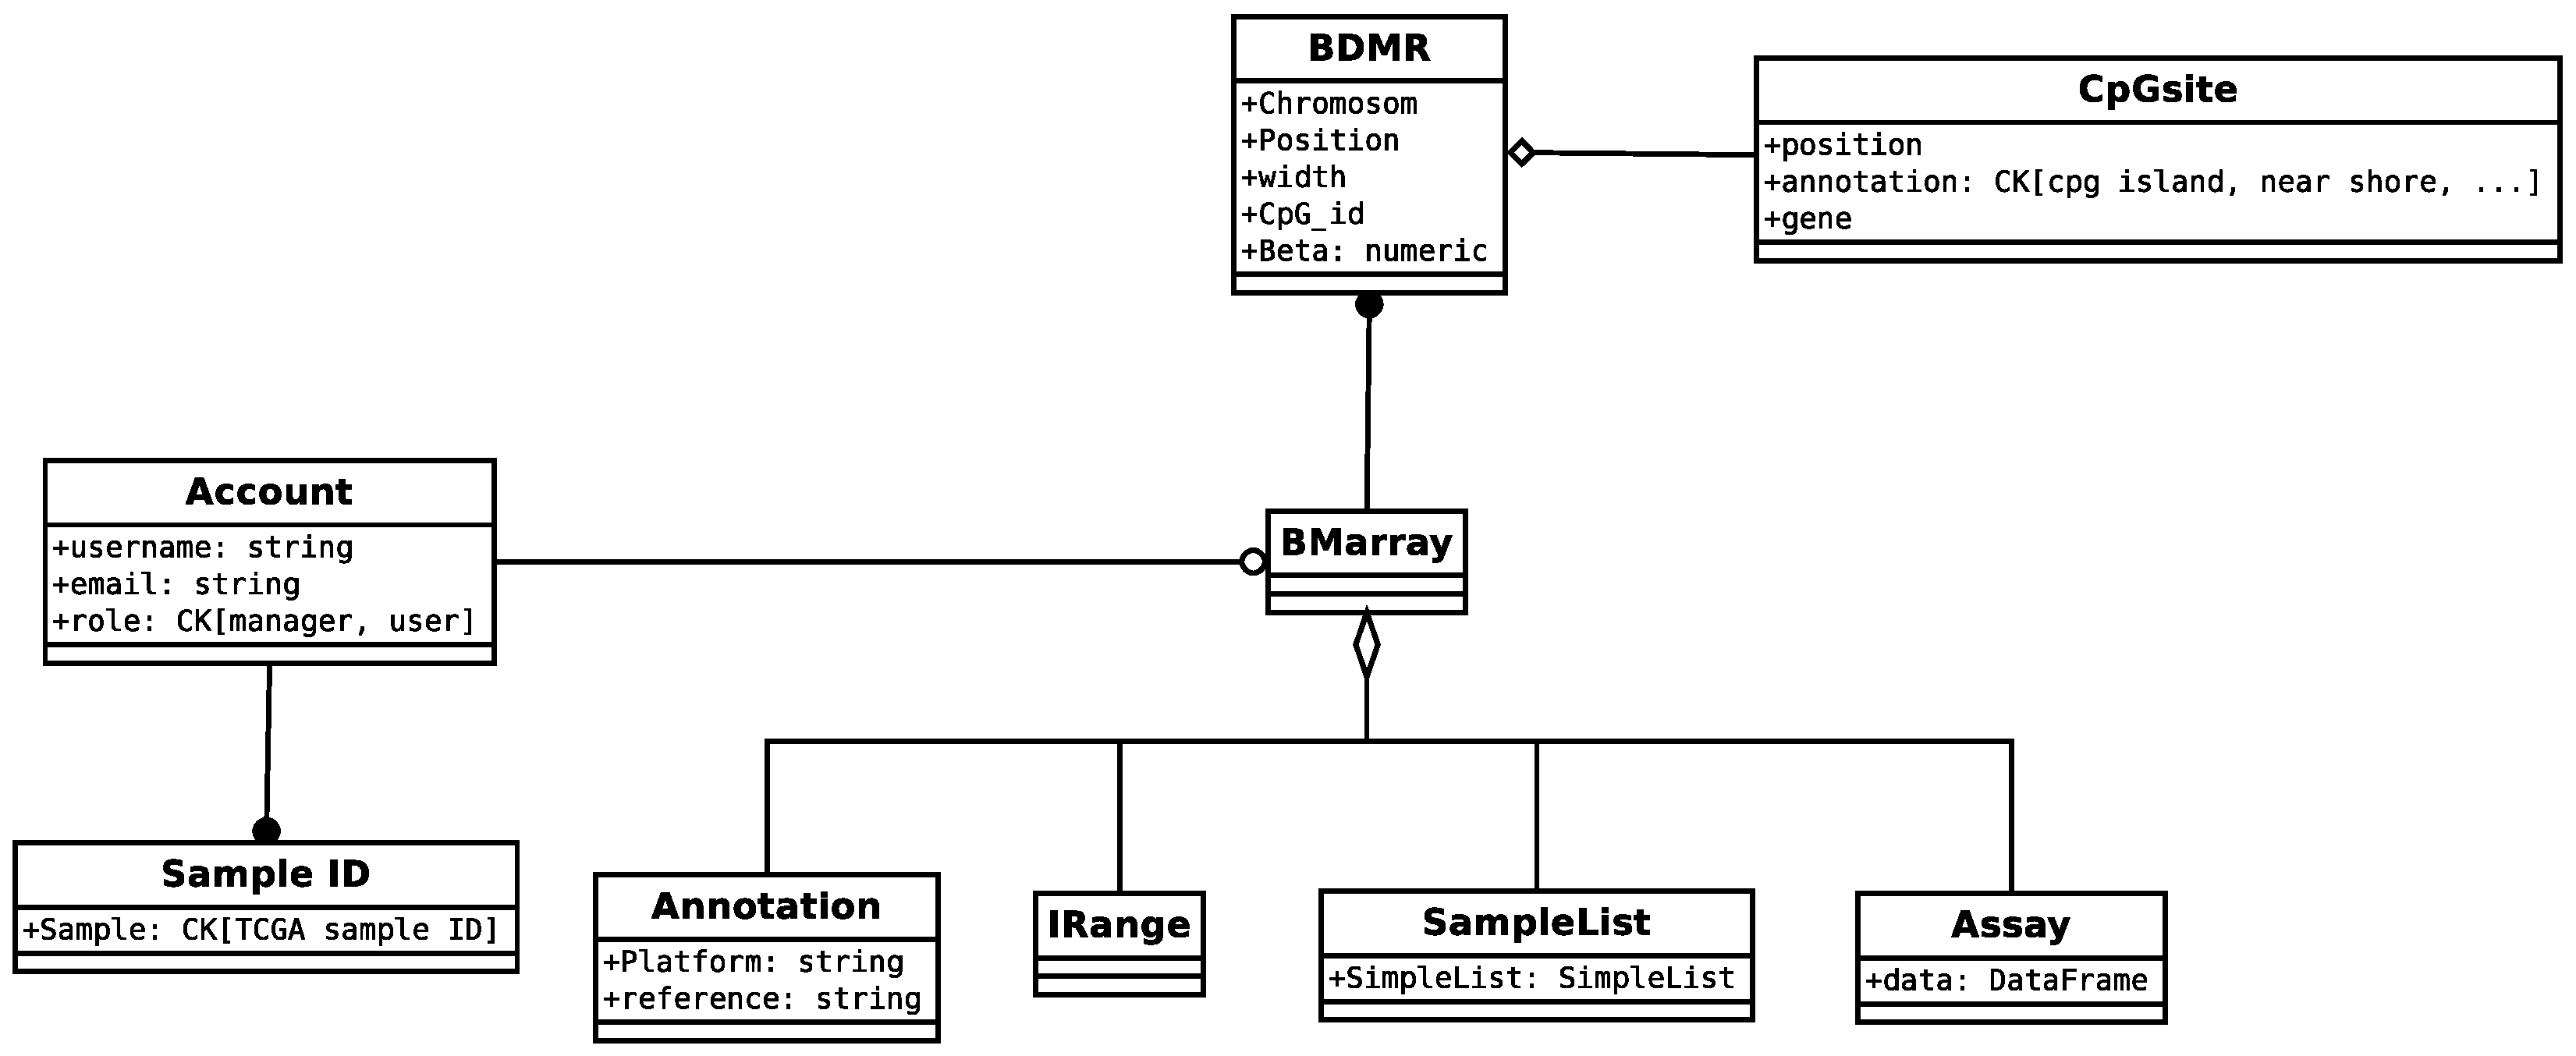
\includegraphics[width=0.8\textwidth]{MethylDB.eps}
\caption{MethylDB's UML object model}
\end{figure}

In our design, we create a data model to communicate with TCGA's Illumina 450K database. Firstly, we create and keep an account object in our MethylDB to store each user's access information. Account object is an object to store each user's original information, besides attributes such as username, password, email, user account object is also connected to several TCGA Illumina 450k sample objects of TCGA. And the 450k sample objects store information of each sample's original 450k microArray information. 

Additionally, our work is an advanced analysis of CpG sites from every account's 450k microArray information dataset, therefore, there exists an association between our comprehensive BMarray object and user account. Once a user creates his account, our system begins to generate a BMarray object based on his account object and TCGA sample object. And the multiplicity of this association is one or zero. It shows that every account has no more than one BMarray comprehensive object. 

After our backend program successfully generates the BMarray object for specific user account, the user account of MethylDB begins to work. And then, we are going to find out all significant DMR(Differential Methylation Region) obejcts by this BMarray object of each account. Since a BMarray is object on whole genome, and each DMR object is cluster of several CpGsites which are closed. In a word, a BMarray object has meveral DMRs objects, and each DMR is build by one or many CpGsites objects. CpGsites object is a description of each CpG site, including attributes such as location, gene name, cpg island id and so on.

All these objects and relationships are described by the model in Figure 1. Based on this model, we can create our MethylDB application.

\section{Result}

\begin{figure}
\centering
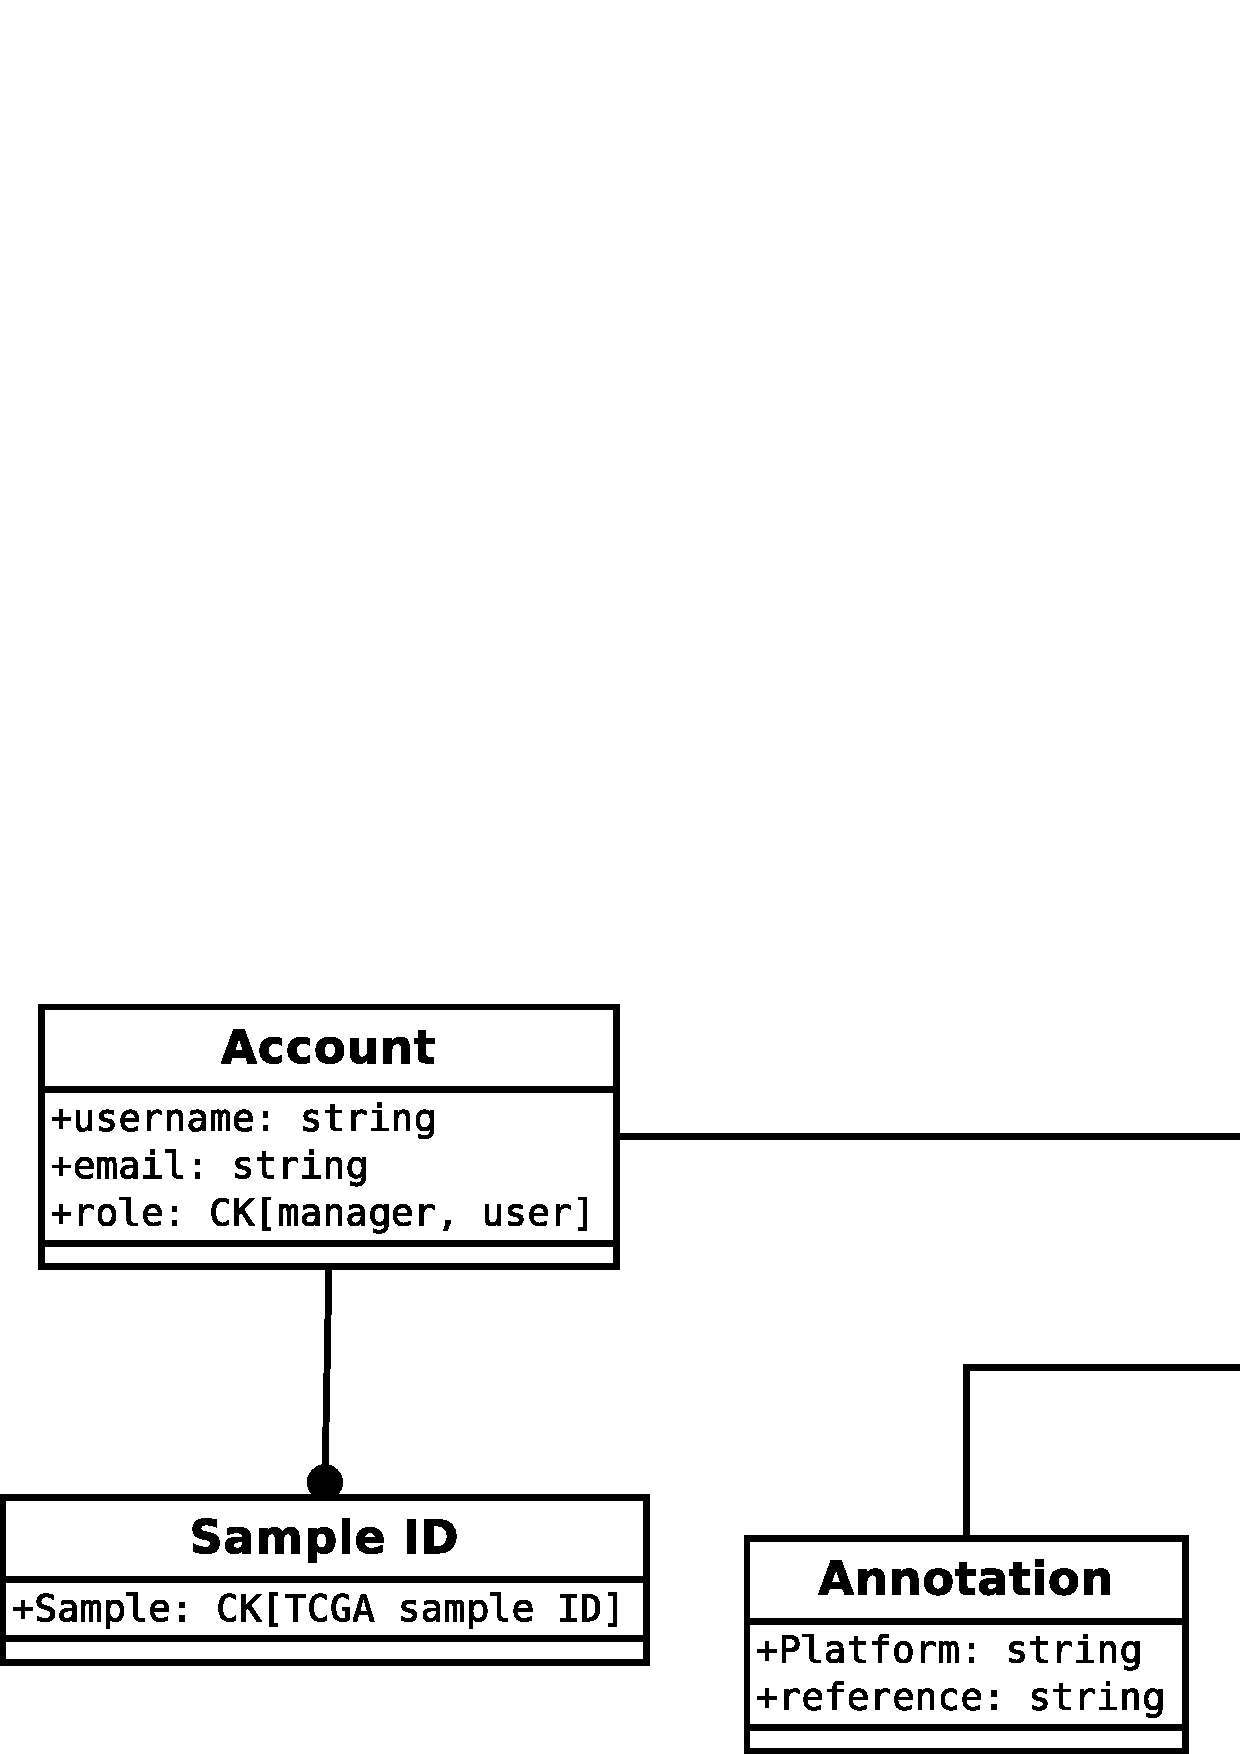
\includegraphics[width=0.8\textwidth]{MethylDB.png}
\caption{Main Interface of MethylDB}
\end{figure}

Figure 2 shows the main page of our MethylDB. Our web application constructed by two panel: one is the side panel which contains log in interface and the other is the main panel which contains different components for different functions.

And our MethylDB has 2 main functions:
\subsection{User account register and login}

\begin{figure}
\centering
\includegraphics[width=0.8\textwidth]{Register.png}
\caption{Register page of MethylDB}
\end{figure}

Register page offers a register entrance of our MethylDB, you need to submit your account's username, password, email and initial TCGA sample ID you prefered to our system. And then, system will help you generate account related BMarray object. And this step is a time consuming step, as the result, our web application will notice you via you email address after we prepare the BMarray object for your account. 

Once user create an account, the system's account database will be modified, we can observed this change in our manager account. 

\begin{figure}
\centering
\includegraphics[width=0.8\textwidth]{Supervisor.png}
\caption{New account registration will insert new user information into account database}
\end{figure}

When user submits his account registration information to MethylDB, system will insert his informaion into account object's database, but the attribute 'status' of the new account is defined as 'processing' and user can not log in his account when his account's status is 'processing', and after BMarray objects generated, user can log in his account. 

\subsection{BMarray object and DMRs object visualization}
There are 3 tabs for BMarray object and DMRs object visualization: 'Statistic' tab is for BMarray's visualization. It show basic information of BMarray object. 

And the the 'Diffbumper' tab is for the DMRs object's visualization, since different BMarray will generate different DMRs set, our MethylDB will help user to generate a beautiful report of $k$ most signifcant DMR from user specific BMarray object. Here, $k$ is the number of DMRs user want to get. 

\begin{figure}
\centering
\includegraphics[width=0.8\textwidth]{Clusterng.png}
\caption{Clustering tab for DMRs object}
\end{figure}

'Clustering' tab is also built for DMRs objects summarization, it will represent each DMR of each sample ID via a heatmap. The heatmap implies DMRs' correlationship. And with the help of clustering heatmap and report about top $k$ significant DMRs, user can find DMRs they are interested in for their future research or diagnosis.


\section{Conclusion}
MethylDB application is created by cooperation between Xin Zhou and Ruichao Hou. Ruichao mainly works for MethylDB's obejct model and Xin mainly works for MethylDB's creation. MethylDB is a database web application and can dynamically respond to user's command. It is also an analysis tool for TCGA database. 

\end{document}
